\chapter{State of the art} \label{sec:colours}

Text-to-image is an emerging field of deep learning where models can generate lifelike and highly detailed images from textual descriptions.  The development of these models is a challenging task that requires the close integration of both computer vision and NLP approaches. The latest advancements in text-to-image models have led to the capability of producing high-quality images with rich semantic content that can now be used for tons of applications including video games and virtual reality, e-commerce, or education among others. Even though recent advancements have allowed the use for commercial applications, generative models remain a challenging and tough problem. This section aims to analyse the current state-of-the-art of text-to-image models

\section{Historical review of text-to-image models}

\section{Diffusion probabilistic models}

Throughout 2022, the capabilities and popularity of text-to-image models have exploded. The general public is aware of some models, such as DALL-E 2, Midjourney, or Stable Diffusion. Nonetheless, the vast majority of people are unaware of the technical prowess required in the field of Artificial Intelligence for these models to exist. This section aims to shed some light on the internal functioning and processes of these models from an academic perspective.

Diffusion probabilistic models are a class of latent variable models that introduce the ideas of nonequilibrium thermodynamics into data generation techniques by homogeneously adding noise into samples. Thus, they join the list of models that manage to generate high-quality images such as variational autoencoders (VAEs) or Generative adversarial networks (GANs). The latter models have been the reference of academic research in recent years and are the benchmark to be surpassed by diffusion models. 

GANs were introduced in 2014 by researchers at the University of Montreal in the paper \textit{Generative Adversarial Nets} \cite{goodfellow2020generative}. The idea is to create generative models through an adversarial process in which two neural networks compete against each other.  One of the networks will be generative while the other will be discriminative. Thus, the generative network will be in charge of capturing the distribution of the training dataset while the discriminative network must distinguish whether a sample comes from the generative network or the training data. The idea is that the generative network maximises the probability that the discriminative network makes errors. 

Diffusion models, on the other hand, achieve high-quality image synthesis results in the paper \textit{Denoising Diffusion Probabilistic Models} \cite{ho2020denoising} by researchers from the University of California, Berkeley. These models are based on creating a Markov chain in which at each step they add Gaussian noise to an image in a diffusion process and then learn to undo it. In this way, a network is trained that is capable of reconstructing images from random noise. The differences between GANs and diffusion models are presented in figure \ref{fig:GansvsDM}.

\begin{figure}
    \centering
    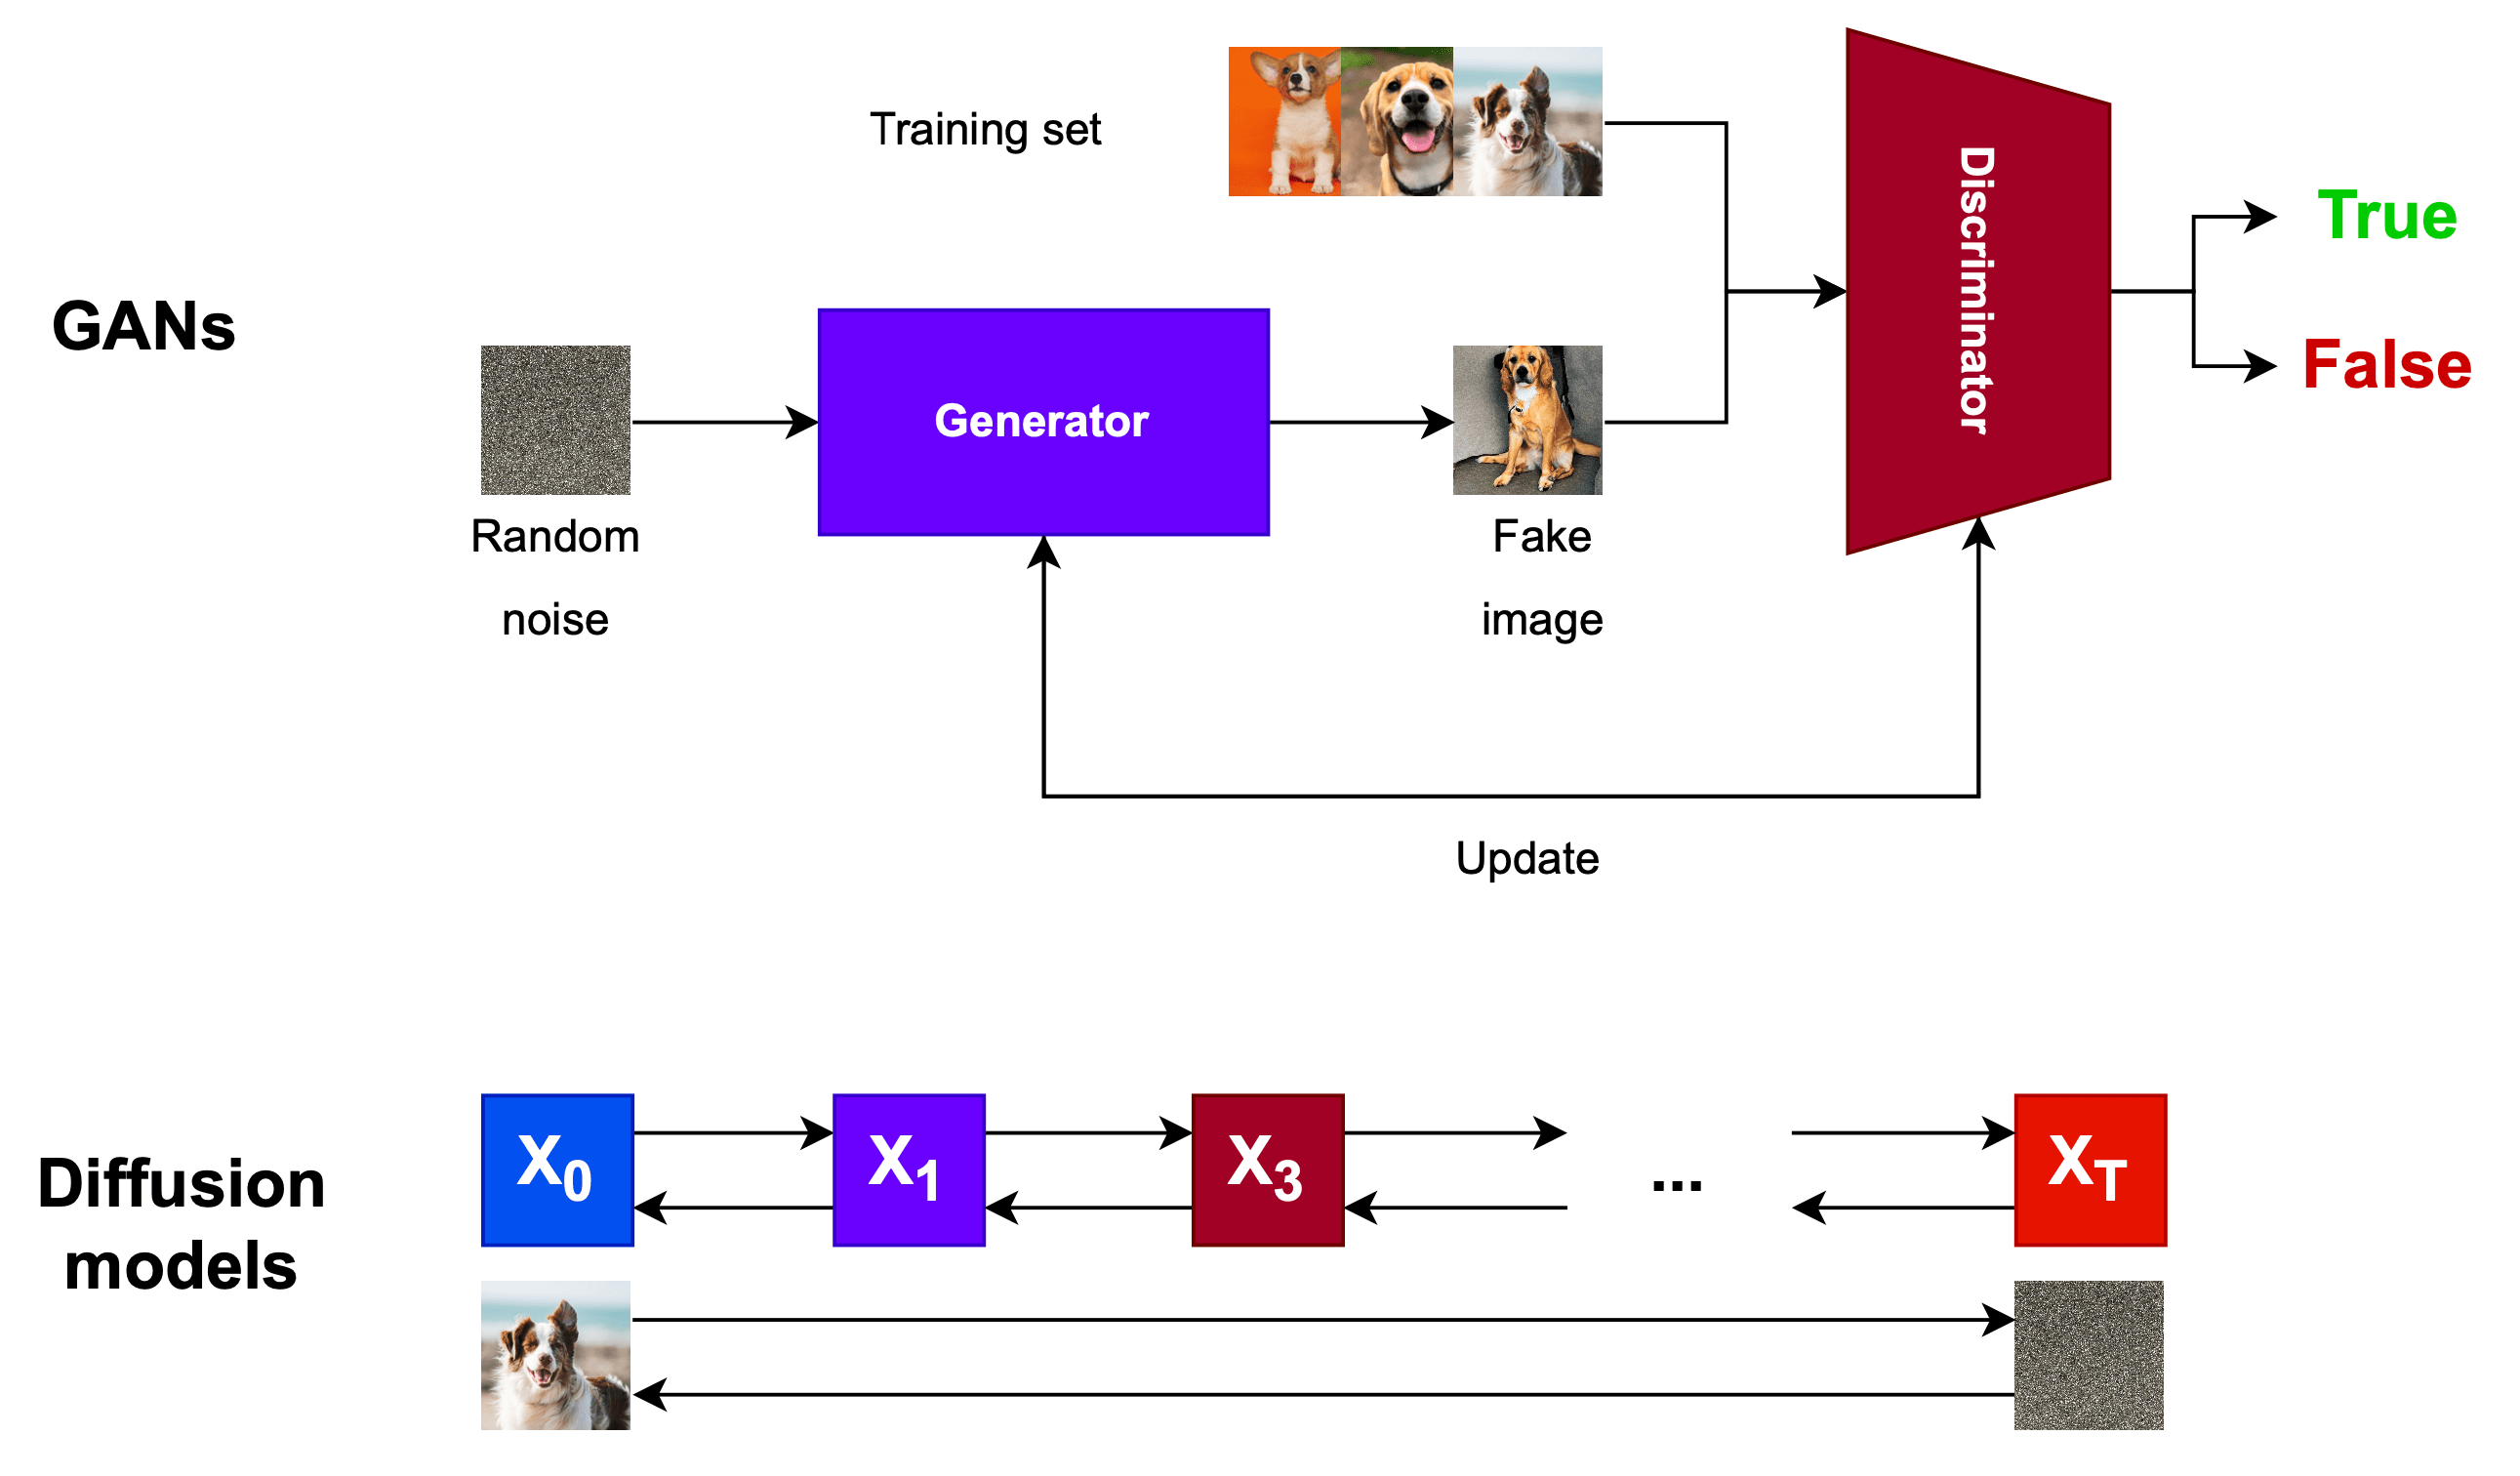
\includegraphics[width=0.75\textwidth]{Pictures/GansvsDM} 
    \caption{Overview of GANs and diffusion models}
    \label{fig:GansvsDM}
\end{figure}

Diving further into the workings of diffusion models, we define the \textbf{forward process} of the Markov chain. The first step is to take a sample of the target data distribution, which we will call $X_0$, and add Gaussian noise in $T$ steps. The forward process is thus defined as a Markov chain in which the state of a sample at time $n$ depends only on the state at time $n-1$. Therefore, one can denote the distribution of any sample conditioned on the initial state $X_0$.

\[ q\left(x_{1:T}\middle| x_0\right)=\prod_{t=1}^{T}{q\left(x_t\middle| x_{t-1}\right)} \]

In every step of the noising process Gaussian noise is added according to some variance schedule $\beta_1...\beta_t$, normally consider as hyperparameters. The restrictions applied to $\beta_t$ are $\beta_1 < \beta_2 ... < \beta_t$ and $\beta_t \epsilon (0, 1)$. $I$ stands for identity.

\[q\left(x_t\middle| x_{t-1}\right)=\mathcal{N}\left(x_t;\sqrt{1-\beta_tx_{t-1}},\beta_tI\right) \]

